\newcommand{\asymcloud}[2][.1]{%
\begin{scope}[#2]
\pgftransformscale{#1}%    
\pgfpathmoveto{\pgfpoint{261 pt}{115 pt}} 
  \pgfpathcurveto{\pgfqpoint{70 pt}{107 pt}}
                 {\pgfqpoint{137 pt}{291 pt}}
                 {\pgfqpoint{260 pt}{273 pt}} 
  \pgfpathcurveto{\pgfqpoint{78 pt}{382 pt}}
                 {\pgfqpoint{381 pt}{445 pt}}
                 {\pgfqpoint{412 pt}{410 pt}}
  \pgfpathcurveto{\pgfqpoint{577 pt}{587 pt}}
                 {\pgfqpoint{698 pt}{488 pt}}
                 {\pgfqpoint{685 pt}{366 pt}}
  \pgfpathcurveto{\pgfqpoint{840 pt}{192 pt}}
                 {\pgfqpoint{610 pt}{157 pt}}
                 {\pgfqpoint{610 pt}{157 pt}}
  \pgfpathcurveto{\pgfqpoint{531 pt}{39 pt}}
                 {\pgfqpoint{298 pt}{51 pt}}
                 {\pgfqpoint{261 pt}{115 pt}}
\pgfusepath{fill,stroke}         
\end{scope}}  

\begin{figure}[!ht]
\centering
\resizebox{1.01\textwidth}{!}{%
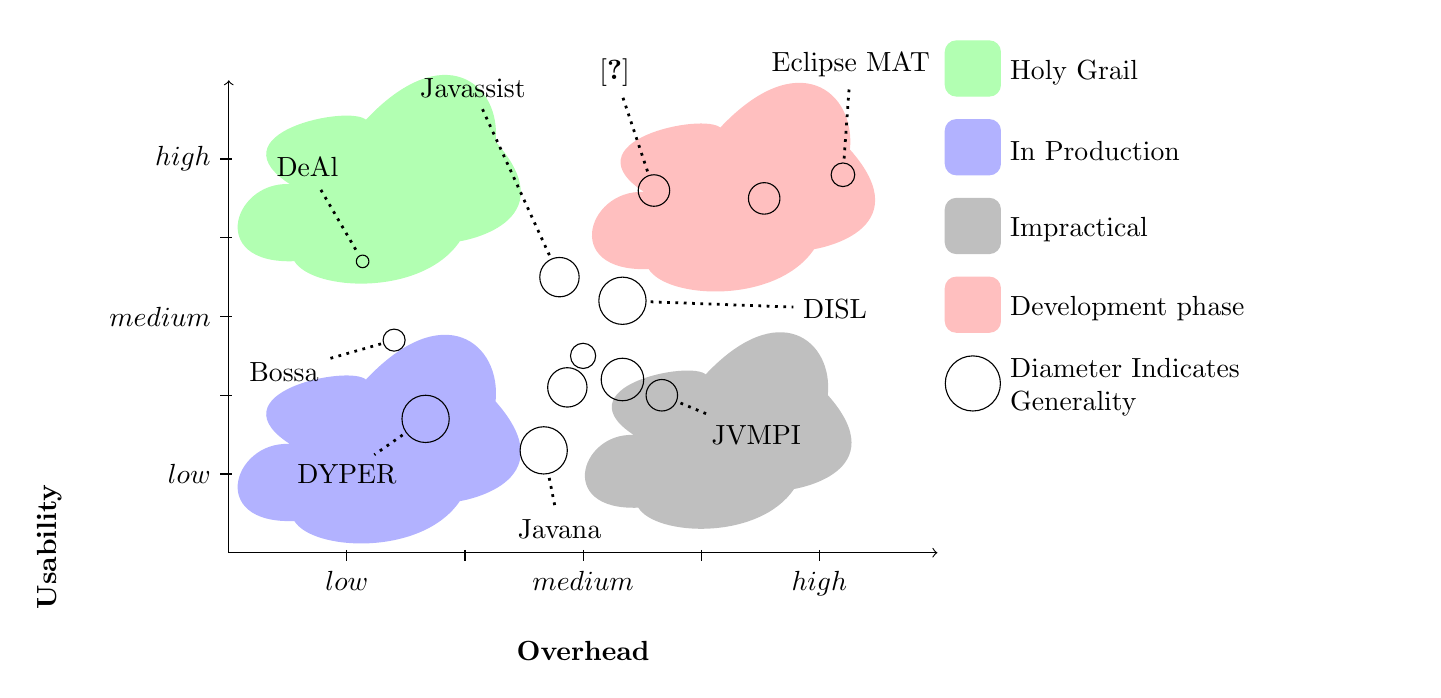
\begin{tikzpicture}
  \draw[->,xshift=0cm] (0,0) -- coordinate (x axis mid) (9,0);
  \draw[->,xshift=0cm] (0,0) -- coordinate (y axis mid) (0,6);
  \foreach \x/\xtext in {1.5/low,3/,4.5/medium,6/,7.5/high}
          \draw [xshift=0cm](\x cm,1pt) -- (\x cm,-3pt)
              node[anchor=north] {$\xtext$};
  \foreach \y/\ytext in {1/low,2/,3/medium,4/,5/high}
          \draw (1pt,\y cm) -- (-3pt,\y cm) node[anchor=east] {$\ytext$}; 
          
  \node[below=1cm] at (x axis mid) {\textbf{Overhead}};
  \node[rotate=90, above left=2cm] at (y axis mid) {\textbf{Usability}};  
  % good region
  \node (cloudgood) at (2,4.9) {\tikz \asymcloud[0.17]{fill=green!30, draw=green!30,thick};};

  %\filldraw[fill=green, draw=green, rounded corners] (0.5,5.5) rectangle (3.5,3);
  
  %bad region
  \node (cloudbad) at (6.3,1.7) {\tikz \asymcloud[0.16]{fill=gray!50, draw=gray!50,thick};};
  
  %useful during development region
  \node (clouddevelopment) at (6.5,4.8) {\tikz \asymcloud[0.17]{fill=pink, draw=pink,thick};};

  %useful in production but not easy to use's region
  \node (cloudproduction) at (2,1.6) {\tikz \asymcloud[0.17]{fill=blue!30, draw=blue!30,thick};};

  % legend
  \filldraw[fill=green!30, draw=green!30, rounded corners] (9.1,6.5) rectangle (9.8,5.8);
  \node[right=0.7cm] at (9.1,6.1) {Holy Grail};
  
  \filldraw[fill=blue!30, draw=blue!30, rounded corners] (9.1,5.5) rectangle (9.8,4.8); 
  \node[right=0.7cm] at (9.1,5.1) {In Production};
  
  \filldraw[fill=gray!50, draw=gray!50, rounded corners] (9.1,4.5) rectangle (9.8,3.8);
  \node[right=0.7cm] at (9.1,4.1) {Impractical};
  
  \filldraw[fill=pink, draw=pink, rounded corners] (9.1,3.5) rectangle (9.8,2.8);
  \node[right=0.7cm] at (9.1,3.1) {Development phase};
  
  \draw (9.45,2.15) circle [radius=0.35];
  \node[right=0.7cm, text width = 5cm, align=left] at (9.1,2.1) {Diameter Indicates\\ Generality};
  
  % very general radius = 0.3
  % general radius = 0.2
  % limited radius = 0.1
  
  % JVMPI - medium usability - high overhead - average generality
  \draw[draw=black] (5.5,2) circle [radius=0.2cm];
  \path (5.5,2) node[circle,minimum size=0.5cm](JVMPI) {}
  		(6.7,1.5) node(JVMPIT) {JVMPI};
  \draw[draw=black,dotted, line width = 1pt] (JVMPI) -- (JVMPIT);
  %\node at (0.5,5.5) {\cite{Liang1999}};
  
  % JAVANA - low usability - medium overhead - high generalidad
  \draw[draw=black] (4,1.3) circle [radius=0.3cm];
  \path (4,1.3) node[circle,minimum size=0.7cm](JAVANA) {}
    		(4.2,0.3) node(JAVANAT) {Javana};
  \draw[draw=black,dotted, line width = 1pt] (JAVANA) -- (JAVANAT);
  
  % Binder CPU Profiling - medium overhead - medium/low usabilityc - low/medium generalidad 
  \draw[draw=black] (4.5,2.5) circle [radius=0.16cm]; % no
  
  % DYPER - medium/low overhead - low usability - high generalidad
  \draw[draw=black] (2.5, 1.7) circle [radius=0.3cm];
  \path (2.5, 1.7) node[circle,minimum size=0.7cm](DYPER) {}
      		(1.5,1) node(DYPERT) {DYPER};
  \draw[draw=black,dotted, line width = 1pt] (DYPER) -- (DYPERT);
  
  % ASM - medium overhead - low/medium usability - high generalidad
  \draw[draw=black] (4.3,2.1) circle [radius=0.25cm]; % [above=0.1]-- (2.3,2.7) node {ASM};
  
  % Javaassist - medium overhead - medium/high usability - high generality
  \draw[draw=black] (4.2,3.5) circle [radius=0.25cm];
  \path (4.2,3.5) node[circle,minimum size=0.6cm](Javassist) {}
        		(3.1,5.9) node(JavassistT) {Javassist};
  \draw[draw=black,dotted, line width = 1pt] (Javassist) -- (JavassistT);
  
  % Profiling with AspectJ - high usability - high overhead - averagage generality
  \draw[draw=black] (6.8,4.5) circle [radius=0.2cm]; % [above=0.1]-- (6.3,5) node {\cite{Pearce:2007:PA:1248445.1248448}};
  
  % Binder Major/AspectJ - medium overhead - high usability - average generalidad
  \draw[draw=black] (5.4,4.6) circle [radius=0.2cm];
  \path (5.4,4.6) node[circle,minimum size=0.5cm](Major) {}
          		(4.9,6.1) node(MajorT) {\cite{Binder:2006:FEM:1173706.1173733}};
  \draw[draw=black,dotted, line width = 1pt] (Major) -- (MajorT);
  
  % DISL - medium overhead - medium usability - full generalidad
  \draw[draw=black] (5,3.2) circle [radius=0.3cm];
  \path (5,3.2) node[circle,minimum size=0.7cm](DISL) {}
        (7.7,3.1) node(DISLT) {DISL};
  \draw[draw=black,dotted, line width = 1pt] (DISL) -- (DISLT);
  
  % Customized aspect weavers - medium overhead - low usability - full generalidad
  \draw[draw=black] (5, 2.2) circle [radius=0.27cm];
  
  % Eclipse MAT/ Visual VM/ YourKit - high overhead - meidum/high usability - limited/medium
  \draw[draw=black] (7.8,4.8) circle [radius=0.15cm];
  \path (7.8,4.8) node[circle,minimum size=0.4cm](Eclipse) {}
        (7.9,6.2) node(EclipseT) {Eclipse MAT};
  \draw[draw=black, dotted, line width = 1pt] (Eclipse) -- (EclipseT);
  
  % DeAl - low overhead - medium/high usability - limited generalidad
  \draw[draw=black] (1.7,3.7) circle [radius=0.08cm];
  \path (1.7,3.7) node[circle,minimum size=0.17cm](DeAl) {}
        (1,4.9) node(DeAlT) {DeAl};
  \draw[draw=black, dotted, line width = 1pt] (DeAl) -- (DeAlT);
  
  % DeAl - low/medium overhead - medium usability - limited generalidad
  \draw[draw=black] (2.1,2.7) circle [radius=0.14cm];
  \path (2.1,2.7) node[circle,minimum size=0.17cm](Bossa) {}
      (0.7,2.3) node(BossaT) {Bossa};
  \draw[draw=black, dotted, line width = 1pt] (Bossa) -- (BossaT);
  
\end{tikzpicture}
}
\caption{\scriptsize Area of circumference indicates how general the approach is (the larger the better)}
\end{figure}
